%%
%% Copyright 2007, 2008, 2009 Elsevier Ltd
%%
%% This file is part of the 'Elsarticle Bundle'.
%% ---------------------------------------------
%%
%% It may be distributed under the conditions of the LaTeX Project Public
%% License, either version 1.2 of this license or (at your option) any
%% later version.  The latest version of this license is in
%%    http://www.latex-project.org/lppl.txt
%% and version 1.2 or later is part of all distributions of LaTeX
%% version 1999/12/01 or later.
%%
%% The list of all files belonging to the 'Elsarticle Bundle' is
%% given in the file `manifest.txt'.
%%

%% Template article for Elsevier's document class `elsarticle'
%% with numbered style bibliographic references
%% SP 2008/03/01
%%
%%
%%
%% $Id: elsarticle-template-num.tex 4 2009-10-24 08:22:58Z rishi $
%%
%%
\documentclass[preprint,12pt,3p]{elsarticle}

%% Use the option review to obtain double line spacing
%% \documentclass[preprint,review,12pt]{elsarticle}

%% Use the options 1p,twocolumn; 3p; 3p,twocolumn; 5p; or 5p,twocolumn
%% for a journal layout:
%% \documentclass[final,1p,times]{elsarticle}
%% \documentclass[final,1p,times,twocolumn]{elsarticle}
%% \documentclass[final,3p,times]{elsarticle}
%% \documentclass[final,3p,times,twocolumn]{elsarticle}
%% \documentclass[final,5p,times]{elsarticle}
%% \documentclass[final,5p,times,twocolumn]{elsarticle}

%% if you use PostScript figures in your article
%% use the graphics package for simple commands
%% \usepackage{graphics}
%% or use the graphicx package for more complicated commands
%% \usepackage{graphicx}
%% or use the epsfig package if you prefer to use the old commands
%% \usepackage{epsfig}

%% The amssymb package provides various useful mathematical symbols
\usepackage{amssymb}
%% The amsthm package provides extended theorem environments
%% \usepackage{amsthm}

%% The lineno packages adds line numbers. Start line numbering with
%% \begin{linenumbers}, end it with \end{linenumbers}. Or switch it on
%% for the whole article with \linenumbers after \end{frontmatter}.
%% \usepackage{lineno}

%% natbib.sty is loaded by default. However, natbib options can be
%% provided with \biboptions{...} command. Following options are
%% valid:

%%   round  -  round parentheses are used (default)
%%   square -  square brackets are used   [option]
%%   curly  -  curly braces are used      {option}
%%   angle  -  angle brackets are used    <option>
%%   semicolon  -  multiple citations separated by semi-colon
%%   colon  - same as semicolon, an earlier confusion
%%   comma  -  separated by comma
%%   numbers-  selects numerical citations
%%   super  -  numerical citations as superscripts
%%   sort   -  sorts multiple citations according to order in ref. list
%%   sort&compress   -  like sort, but also compresses numerical citations
%%   compress - compresses without sorting
%%
%% \biboptions{comma,round}

% \biboptions{}

\usepackage{graphicx}
\usepackage[space]{grffile}
\usepackage{latexsym}
\usepackage{amsfonts,amsmath,amssymb}
\usepackage{url}
\usepackage[utf8]{inputenc}
\usepackage{fancyref}
\usepackage{hyperref}
\hypersetup{colorlinks=false,pdfborder={0 0 0},}

\newcommand{\truncateit}[1]{\truncate{0.8\textwidth}{#1}}
\newcommand{\scititle}[1]{\title[\truncateit{#1}]{#1}}
\usepackage{listings}
\usepackage{comment}
\newcommand{\unit}[1]{\ensuremath{\, \mathrm{#1}}}

\newcommand{\aj}{AJ}			% Astronomical Journal
\newcommand{\araa}{ARA\&A}		% Annual Review of Astron and Astrophys
\newcommand{\apj}{ApJ}			% Astrophysical Journal
\newcommand{\apjl}{ApJLett}		% Astrophysical Journal, Letters
\newcommand{\apjlett}{ApJLett}		% Astrophysical Journal, Letters
\newcommand{\apjs}{ApJS}		% Astrophysical Journal, Supplement
\newcommand{\apjsupp}{ApJS}		% Astrophysical Journal, Supplement
\newcommand{\ao}{Appl.~Opt.}		% Applied Optics
\newcommand{\apss}{Ap\&SS}		% Astrophysics and Space Science
\newcommand{\aap}{A\&A}			% Astronomy and Astrophysics
\newcommand{\astap}{A\&A}		% Astronomy and Astrophysics
\newcommand{\aapr}{A\&A~Rev.}		% Astronomy and Astrophysics Reviews
\newcommand{\aaps}{A\&AS}		% Astronomy and Astrophysics, Supplement
\newcommand{\azh}{AZh}			% Astronomicheskii Zhurnal
\newcommand{\baas}{BAAS}		% Bulletin of the AAS
\newcommand{\jrasc}{JRASC}		% Journal of the RAS of Canada
\newcommand{\memras}{MmRAS}		% Memoirs of the RAS
\newcommand{\mnras}{MNRAS}		% Monthly Notices of the RAS
\newcommand{\pra}{Phys.~Rev.~A}		% Physical Review A: General Physics
\newcommand{\prb}{Phys.~Rev.~B}		% Physical Review B: Solid State
\newcommand{\prc}{Phys.~Rev.~C}		% Physical Review C
\newcommand{\prd}{Phys.~Rev.~D}		% Physical Review D
\newcommand{\pre}{Phys.~Rev.~E}		% Physical Review E
\newcommand{\prl}{Phys.~Rev.~Lett.}	% Physical Review Letters
\newcommand{\pasp}{PASP}		% Publications of the ASP
\newcommand{\pasj}{PASJ}		% Publications of the ASJ
\newcommand{\qjras}{QJRAS}		% Quarterly Journal of the RAS
\newcommand{\revmodphys}{Rev.\ Mod.\ Phys.} %Rev Mod Phys
\newcommand{\skytel}{S\&T}		% Sky and Telescope
\newcommand{\solphys}{Sol.~Phys.}	% Solar Physics
\newcommand{\sovast}{Soviet~Ast.}	% Soviet Astronomy
\newcommand{\ssr}{Space~Sci.~Rev.}	% Space Science Reviews
\newcommand{\zap}{ZAp}			% Zeitschrift fuer Astrophysik
\newcommand{\nat}{Nature}		% Nature
\newcommand{\iaucirc}{IAU~Circ.}       	% IAU Circulars
\newcommand{\aplett}{Astrophys.~Lett.} 	% Astrophysics Letters
\newcommand{\apspr}{Astrophys.~Space~Phys.~Res.}% Astrophysics Space Physics Research
\newcommand{\fcp}{Fund.~Cosmic~Phys.}  % Fundamental Cosmic Physics
\newcommand{\gca}{Geochim.~Cosmochim.~Acta}   % Geochimica Cosmochimica Acta
\newcommand{\grl}{Geophys.~Res.~Lett.} % Geophysics Research Letters
\newcommand{\jcp}{J.~Chem.~Phys.}	% Journal of Chemical Physics
\newcommand{\jgr}{J.~Geophys.~Res.}	% Journal of Geophysics Research
\newcommand{\nphysa}{Nucl.~Phys.~A}   % Nuclear Physics A
\newcommand{\physrep}{Phys.~Rep.}   % Physics Reports
\newcommand{\physscr}{Phys.~Scr}   % Physica Scripta
\newcommand{\planss}{Planet.~Space~Sci.}   % Planetary Space Science
\newcommand{\procspie}{Proc.~SPIE}   % Proceedings of the SPIE

\usepackage{relsize}
\newcommand\Cpp{C\nolinebreak[4]\hspace{-.05em}\raisebox{.4ex}{\relsize{-3}{\textbf{++}}}}


\definecolor{midgray}{gray}{0.85}%

\usepackage{listings}


\lstdefinestyle{code}{%
     basicstyle=\footnotesize\ttfamily,       
     frame=single,               
     framesep=1pt,               
     framerule=0.8pt,            
     rulecolor=\color{midgray},  
     breaklines=true,           
     breakindent=0pt,
     backgroundcolor=\color{midgray},
     prebreak=\mbox{\textbackslash{}}             
}

\lstdefinestyle{python}{
  style=code,
  belowcaptionskip=1\baselineskip,
  breaklines=true,
  frame=single,
  framesep=2pt,
  xleftmargin=\parindent,
  language=Python,
  showstringspaces=false,
  basicstyle=\footnotesize\ttfamily,
  keywordstyle=\bfseries\color{green!40!black},
  commentstyle=\itshape\color{gray},
  identifierstyle=\color{black},
  stringstyle=\color{gray},
  rulecolor=\color{midgray}, 
}

\lstdefinestyle{java}{
  style=python,
  language=Java
}





\journal{Elsevier Journal}

\begin{document}

\begin{frontmatter}

%% Title, authors and addresses

%% use the tnoteref command within \title for footnotes;
%% use the tnotetext command for the associated footnote;
%% use the fnref command within \author or \address for footnotes;
%% use the fntext command for the associated footnote;
%% use the corref command within \author for corresponding author footnotes;
%% use the cortext command for the associated footnote;
%% use the ead command for the email address,
%% and the form \ead[url] for the home page:
%%
%% \title{Title\tnoteref{label1}}
%% \tnotetext[label1]{}
%% \author{Name\corref{cor1}\fnref{label2}}
%% \ead{email address}
%% \ead[url]{home page}
%% \fntext[label2]{}
%% \cortext[cor1]{}
%% \address{Address\fnref{label3}}
%% \fntext[label3]{}

\title{Iris: Build and Analyze Broadband Spectral Energy Distributions}


\author[first]{Omar Laurino}
\address[first]{Smithsonian Astrophysical Observatory}

 
\author[0]{Jamie Budynkiewicz}
\address[0]{Smithsonian Astrophysical Observatory}
 
\author[1]{Janet Evans}
\address[1]{Smithsonian Astrophysical Observatory}




\begin{abstract}
The abstract goes here

\end{abstract}




%\begin{keyword}
%% keywords here, in the form: keyword \sep keyword

%% MSC codes here, in the form: \MSC code \sep code
%% or \MSC[2008] code \sep code (2000 is the default)

%\end{keyword}

\end{frontmatter}

\bibliographystyle{elsarticle-num}


\label{sec:introduction}
\section{Introduction} 
The International Virtual Observatory Alliance~\citep{2004SPIE.5493..137Q} provides a set of standards and protocols that enable interoperability among astronomy-centered services and applications.
%Building VO-enabled, interoperable applications poses several challenges to software developers.
In order to design effective applications, one wants to leverage Virtual Observatory (VO) standards and protocols without exposing the complexity and technicality of their specifications to the users. Also, while application developers implement many desired functionalities, they must keep the door open for plugging in user's analysis code, and allow third party developers to extend the application's functionality without being aware of the standards themselves.

Designing such general purpose applications thus becomes an exercise in designing a framework that implements some basic, effective functionality for a wide set of use cases, while being highly extensible.

Iris, the Virtual Astronomical Observatory\footnote{www.usvao.org}~\citep{2012SPIE.8449E..0HB} spectral energy distribution (SED) analysis tool, is such a VO-enabled application. Iris was developed to provide the astronomical community with a desktop application for building, viewing and analyzing broadband spectro-photometric SEDs, while implementing VO standards and protocols and taking advantage of existing astronomy software \citep{2012ASPC..461..893D,2013AAS...22124038L}.

Users may populate SEDs with data from files, built-in portals to data archives, and other VO applications. Iris is lenient on the data format, so while it natively supports VO-compliant files (properly annotated VOTABLE and FITS files), Iris can ingest ASCII, CSV, and other table-like formats with some user input. Iris also provides interactive data visualization and editing tools, and a SED fitting tool for fine-tuned modeling. Users may choose from a suite of provided astrophysical models, or load their own Python functions and template libraries. All front-end features of Iris completely hide the underlying technical VO standards and protocols from the user.

Iris was devoted to provide functionality in a specific scientific domain, namely the analysis of broad-band SEDs. This requirement clearly defines the semantic scope of the  Iris extensible framework, and provides a clear abstraction layer to both users and developers, inside and outside of the development team.

In this paper we present the Iris application, software design, and the built-in infrastructure to support application extensibility with plug-ins. In section \ref{sec:overview} we briefly explore the landscape of SED applications and analysis tools which Iris joined. An overview of Iris' general architecture (the Iris \emph{stack}) is illustrated in section \ref{sec:stack}. We introduce the Iris features in section \ref{sec:builtin}, and explore how astronomers can include their own models or templates as Python functions in section \ref{sec:usermodels}. We provide details of the Iris extensible framework design (section \ref{sec:architecture}), followed by a detailed description of the more advanced Iris functionalities (section \ref{sec:components}). Finally, we include a ``How-to'' description about extending Iris using plug-ins (section \ref{sec:plugins}).

\section{SED Analysis: an overview}
\label{sec:overview}

Fitting spectral energy distributions allows astronomers to estimate fundamental physical properties like stellar mass, star formation rates, dust content and overall environments of astronomical objects (e.g. \citet{1998AJ....115.1329S}, \citet{2001ApJS..137..139S}, \citet{2007ApJS..169..328R}, and many others). With deeper wide-field surveys and increasing numbers of datasets over the years, astronomers have been able to utilize multi-wavelength SEDs more frequently for their research. As such, many robust SED analysis codes have been created to help astronomers model, fit, and derive physical quantities from SEDs \citep{2011Ap&SS.331....1W,2013ARA&A..51..393C}. These widely-used codes implement a diverse set of methods, for instance: inversion (\texttt{PAHFIT} \citep{2007ApJ...656..770S}, \texttt{STARLIGHT} \cite{2004MNRAS.355..273C}), principal component analysis \citep{2009MNRAS.394.1496B}, $\mathrm{\chi}^{2}$-minimization codes (\texttt{Le Phare} \citep{1999MNRAS.310..540A}, \texttt{hyperz} \citep{2000A&A...363..476B}), and Bayesian inference (\texttt{GalMC} \citep{2011ApJ...737...47A}; \texttt{VOSA} \citep{2008A&A...492..277B}; \texttt{BPZ} \citep{2000ApJ...536..571B}).

Most distributed fitting packages are tailored for specific data sets or spectral ranges (e.g. PAHFIT, STARLIGHT), providing robust fitting methods and results. They require the data to be in a specific format with specific units in order for the tool to work properly. When fitting a broadband SED that spans over decades in the spectrum, the astronomer will typically gather data from different public archives and colleagues to add to their own dataset. More often than not, the datasets are presented in different file formats and units. The user must provide their own methods to extract the necessary data from each file, convert the units, and output a file in the single format supported by the tool. 

%The astronomer may also want to inspect the SED, for example plotting it against different units, normalizing some of points or spectral segments, shifting the SED to another redshift, and performing other simple visualization tasks.

While SED analysis tools have input formats that may be different from each other, they nevertheless require effectively the same information to run. It thus becomes a matter of providing an interoperable framework that makes building, viewing, and analyzing SEDs a straightforward process.

% However, most SED analysis tools require similar data and pre-processing steps, like gathering and converting the data to compliant formats for the tools. Thus it becomes only a matter of providing an interoperable framework that makes building, viewing, and analyzing SEDs a straightforward process.

Following VO efforts to seamlessly combine data services and applications, Iris offers a standard means of building large broadband SEDs from different sources in various data formats, while providing robust fitting methods and interactive visualization capabilities. Users can input SED data from a local file or a URL, with high leniency on the data format. Users may also beam data from other VO-enabled applications or data archive services through SAMP (Simple Application Messaging Protocol; \citet{2011arXiv1110.0528T}). If the data format follows the IVOA Spectrum Data Model v1.03 \citep{2012arXiv1204.3055M}, or in other words a VO-compliant VOTable or FITS file, the data is read-in without any input by the user; otherwise, the user supplies the units and mapping to the spectral-flux coordinates in the file. How this method works is described in Section \ref{sec:components}.

%While each code is tailored for specific datasets or object types, most SED analysis tools share similar necessities and require the same pre-processing steps. Thus it is worth developing an interoperable SED tool that Following VO efforts to seamlessly combine data services and applications, Iris offers a standard means of building large broadband SEDs from different sources in various data formats, while providing robust fitting methods and interactive visualization capabilities.

%[FIX ME: make me a happy, positive statement] While these exacting steps are worthwhile for the quality fitting results, gathering, pre-processing, and converting data to plug it in to a fitting engine should be standard/interpoerable and straightfoward. 

%This inconvenience -- building SEDs from multiple sources -- drove a part of Iris' SED analysis design. Following VO efforts to seamlessly combine data services and applications, Iris offers a standard means of building large broadband SEDs from different sources in various data formats, while providing robust fitting methods and interactive visualization capabilities. Users can input SED data from a local file or a URL, with high leniency on the data format. Users may also beam data from other VO-enabled applications or data archive services through SAMP (Simple Application Messaging Protocol; \citet{2011arXiv1110.0528T}). If the data format follows the IVOA Spectrum Data Model v1.03 \citep{2012arXiv1204.3055M}, or in other words a VO-compliant VOTable or FITS file, the data is read-in without any input by the user; otherwise, the user supplies the units and  mapping to the spectral-flux coordinates in the file. How this method works is described in Section \ref{sec:components}.

Iris is meant to be an open box SED analysis tool. If Iris is missing certain functionality, the user may develop a plugin for that functionality and add it to Iris. Thus, a user can employ Iris' SED building capabilites while running custom analysis, which in theory could be one of the fitting packages discussed above. We explore this possibility in detail in Section \ref{sec:plugins}

%Users can input SED data from a local file, a URL, another VO-enabled application, or directly from VO-enabled data archive services, with high leniency on the data format.

%\begin{comment}
%Following the VO effort for seamless interoperability between data services and applications,  

%The Virtual Observatory is an effort to standardize data formats and services so that users can seamlessly exchange data back and forth between archives and applications.  
%
%Iris offers a standard means of building large broadband SEDs from different sources in various data formats, while providing robust fitting methods and interactive visualization capabilities.
%\end{comment}

\section{The Iris Stack}
\label{sec:stack}

\begin{figure}[h!]
\begin{center}
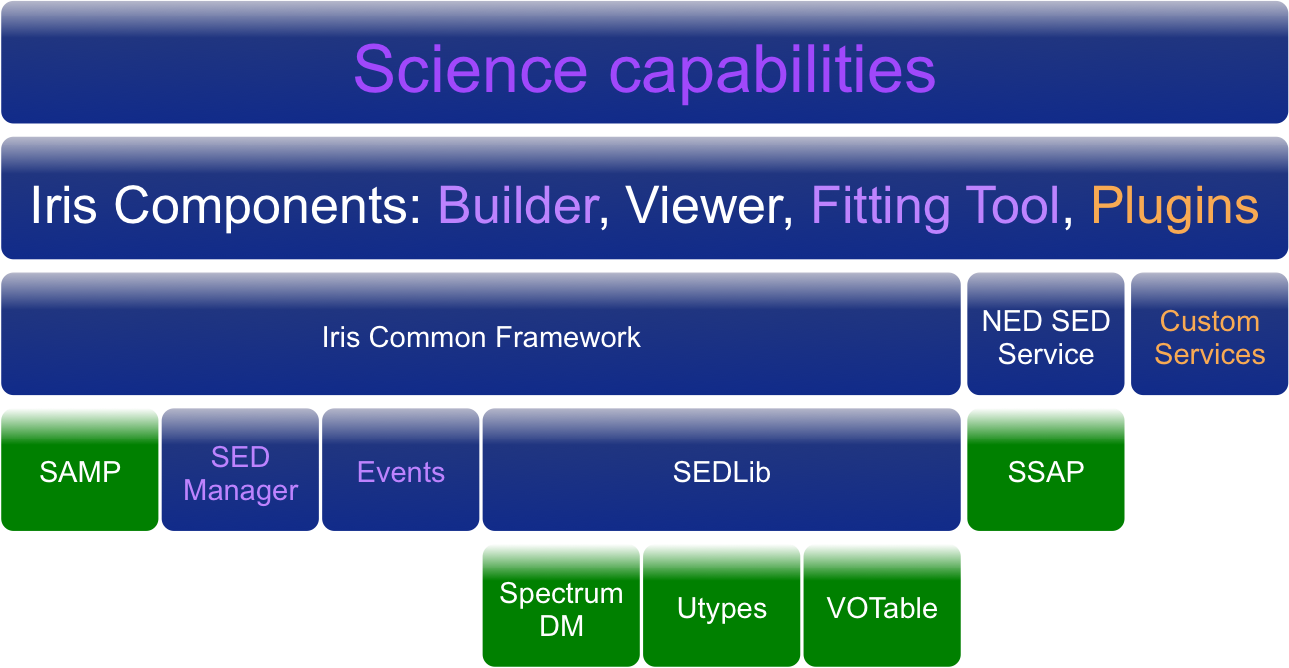
\includegraphics[width=0.7\columnwidth]{figures/IrisStack/IrisStack.png}
\caption{\textbf{\label{fig:stack} The Iris Stack} Iris employs an extensible, loosely coupled architecture that allows developers to create components using a common set of abstraction layers on top of web services, desktop applications using SAMP, and Virtual Observatory standards and protocols.}
\end{center}
\end{figure}

The Iris stack (Figure \ref{fig:stack}) shows how one can put the cold and technical IVOA specifications to work for scientists through higher and higher layers of abstraction: the technical details of the Virtual Observatory standards and protocols lie in the bottommost layers, the internals of the Iris building blocks lie in the middle layers, while the topmost layers express high-level user-oriented functionalities.

A reader without any knowledge of programming, let alone of the VO specifications, should understand the labels used in the topmost layers of the diagram and their components (e.g. the Fitting Tool, Redshift), as long as they have some knowledge of astronomical SEDs.

On the other hand, a developer would find words like framework, service, and manager quite familiar, while it takes a VO-savvy person to decode the acronyms at the bottom of the diagram.

This fact reflects the different entry points for the different audiences of the application: core developers work at all levels of the stack, but need to lay out the foundations on top of the standard specifications; third party developers use the middle-level abstractions offered by the Iris framework, while end users can limit their interaction to familiar astronomical concepts through the application's user interface. End users can also plug in their modeling code and upload templates libraries to Iris.

The color code in Figure \ref{fig:stack} adds a different dimension to this diagram and taps into a different characteristic of the Iris architecture: extensibility. In particular, blue boxes with purple letters denote extensible components of the architecture, i.e. component that offer hooks into the Iris architecture to users and developers. The orange labels, on the other hand, express components that were not even part of the Iris design, but that can be loaded in Iris as plug-ins, possibly providing an interface to access non-standard services. Some of these plug-ins, along with a description of the design of the Iris Software Development Kit, will be introduced in section \ref{sec:plugins}.

The Iris development team also faced some extra challenges: our team was distributed in nature, with developers and managers working from different institutions with different tools and practices \citep{2012SPIE.8449E..0IE}. Moreover, willing to reuse existing software instead of reinventing the proverbial wheel, we had to integrate different existing software components in a seamless way.

In summary, the Iris framework, which we will describe more in detail in the following sections, was designed to address several different requirements:
\begin{itemize}
\item functional requirements gathered by the Iris team's lead scientists;
\item functional requirements unknown at development-time;
\item the distributed nature of the Iris development team;
\item the willingness to bring existing tools and services together in a single application.
\end{itemize}

The Iris stack offers a non-technical view of the Iris architecture and design. While it shows effectively how we tried to abstract end users and developers from the VO specifications and from the specifics of the Iris internals, it does not express the technical solutions that we employed to achieve such extensible architecture and to meet the aforementioned requirements: more details about the Iris built-in features and how they can be extended will be provided in the following sections.

\section{Built-in functionality}
\label{sec:builtin}

In this section, we go through a specific use-case of Iris to showcase its main functionalities. We build, inspect, and fit a SED of the flat radio spectrum quasar (FRSQ) blazar PKS 1127-14, and save our results to file. In Section \ref{sec:components}, we describe how these functions work in terms of the Iris stack.

\subsection{Building the SED}

As stated in Section \ref{sec:overview}, Iris can read data from a variety of sources in different formats. Figure \ref{fig:load_data} shows an example session of loading data into Iris. The user loads PLANCK data in the form of an ASCII spectrum file (where there is a column for the spectral, flux, and flux errors) and a photometry catalog-style SAMP message of WISE data from TOPCAT \citep{2005ASPC..347...29T}. When Iris receives data in non-VO compliant formats, Iris opens file reader GUIs in which the user provides the mapping for the spectral, flux and flux uncertainties. The file importers provide helpful hints for the user when filling in the forms.

Wanting to analyze the entire SED of the blazer, the user queries the NED database for photometric data through the NED SED Service\footnote{http://vo.ned.ipac.caltech.edu/SED\_Service/} portal in Iris. The data is automatically added to the SED Builder and the display. The user then opens the ASDC\footnote{http://www.asdc.asi.it/} query tool, which provides more control over the data being added to the plot; she types the target name, chooses observation date ranges, selects optical/UV data from SWIFT and GALEX (see Figure~\ref{fig:load_data}), and imports the data to the SED.

\subsection{Inspecting the SED}

With all of the data uploaded, the user may switch the spectral and flux units; Iris takes care of all unit conversions once the data is read in. Before starting a fitting session, the she wants to remove from the SED data without flux uncertainty measurements. The user opens the Metadata Browser from the plotting display (SED Viewer), switches to the Data tab, and types a Python-expression into the Boolean filter to highlight the points whose error measuments are above 0 (i.e. points that have uncertainty measurements). With the desired data points hilgihted in the window, the user clicks ``Create new SED;'' this adds another SED to the SED Builder, which is managed separately from our original dataset.

At this point, the user chooses to shift the SED to restframe. PKS 1127-14 is at redshift $z=1.18$. The user opens up the Science tool by clicking the ``Shift, Interpolate, Integrate'' icon on the Iris desktop; under ``Redshift,'' she types $1.18$ into the Initial field, and leaves 0 in the Final box, finally creating a new SED in the restframe.

The user decides to save the SED they built to a file. SEDs are saved in VO-compliant FITS or VOTable formats which can be re-read into Iris or other programs (e.g. TOPCAT; IDL or Python interpreters). Users can save all of the metadata associated with the SEDs, or choose to save just the spectral, flux and flux uncertainties in a simplier format.

\subsection{Fitting the SED}

%Blazar SEDs are dominated by two peaks. The lower energy features can be explained by radio synchrotron radiation from the relativistic electrons in a jet pointing at our line-of-sight and inverse Compton scattering off the synchrotron photons or photons from the originating environment. Massaro et al. (2006) and Tramacere et al. (2007) have shown that both emission processes can be modeled by log-parabolic distributions. In FRSQ blazars, the radio emission is weaker, and so other features, like the accretion disk surrounding the  
Blazar SEDs are dominated by two peaks. It has been shown that the low-energy peak, due to radio synchrotron radiation, and the higher-energy bump, due to inverse Compton radiation, can be modeled by log-parabolic distributions \citep{2006A&A...448..861M,2009A&A...501..879T}. Also present in blazars are an accretion disk and a hot dusty torus surrounding the super-massive black hole, both of which can be modeled by blackbody distributions \citep{2002ApJ...575..667D}. The user will linearly combine these four models to fit the multi-wavelength SED of PKS 1127-14.  

The user starts a fitting session by opening the Fitting Tool component on the Iris desktop. The SED Viewer updates with an overplotted, unfit powerlaw model, and a plot of the residuals shown below the data. The user removes the powerlaw component, and adds four models from the Preset Components provided by Sherpa: two logarithmic parabolas (\texttt{logparabola}s) for the radio synchrotron and inverse Compton radiation and two blackbodies (\texttt{blackbody}s) for the hot dust and accretion disk. The models are added to the Components field, where the model parameter values are displayed. Double-clicking a component allows you to edit the parameters, e.g. freeze and thaw parameters, reset their initial values, and set their minimum and maximum values. 

In the Model Expression field, the components are combined in arbitrary ways. Each component is given an ID which is used to reference the component in the Model Expression field. The user can also set the data ranges to be fit. In this example, we linearly combine the models, adding and fitting them one-by-one, defining the data ranges for each component, then freezing the component afterwards. For each fit, we use Neldermead optimization and least squares as the statistic. We thaw all components and refit the entire SED; the result is shown in Figure \ref{fig:fitting1}. 

The user saves the fit results to a text file, showing the fit statistics, model used, and the best-fit parameter values. She can also save an XML-style file of the model that can be re-read into Iris and fit to other SED data.

\begin{figure}[h!]
\begin{center}
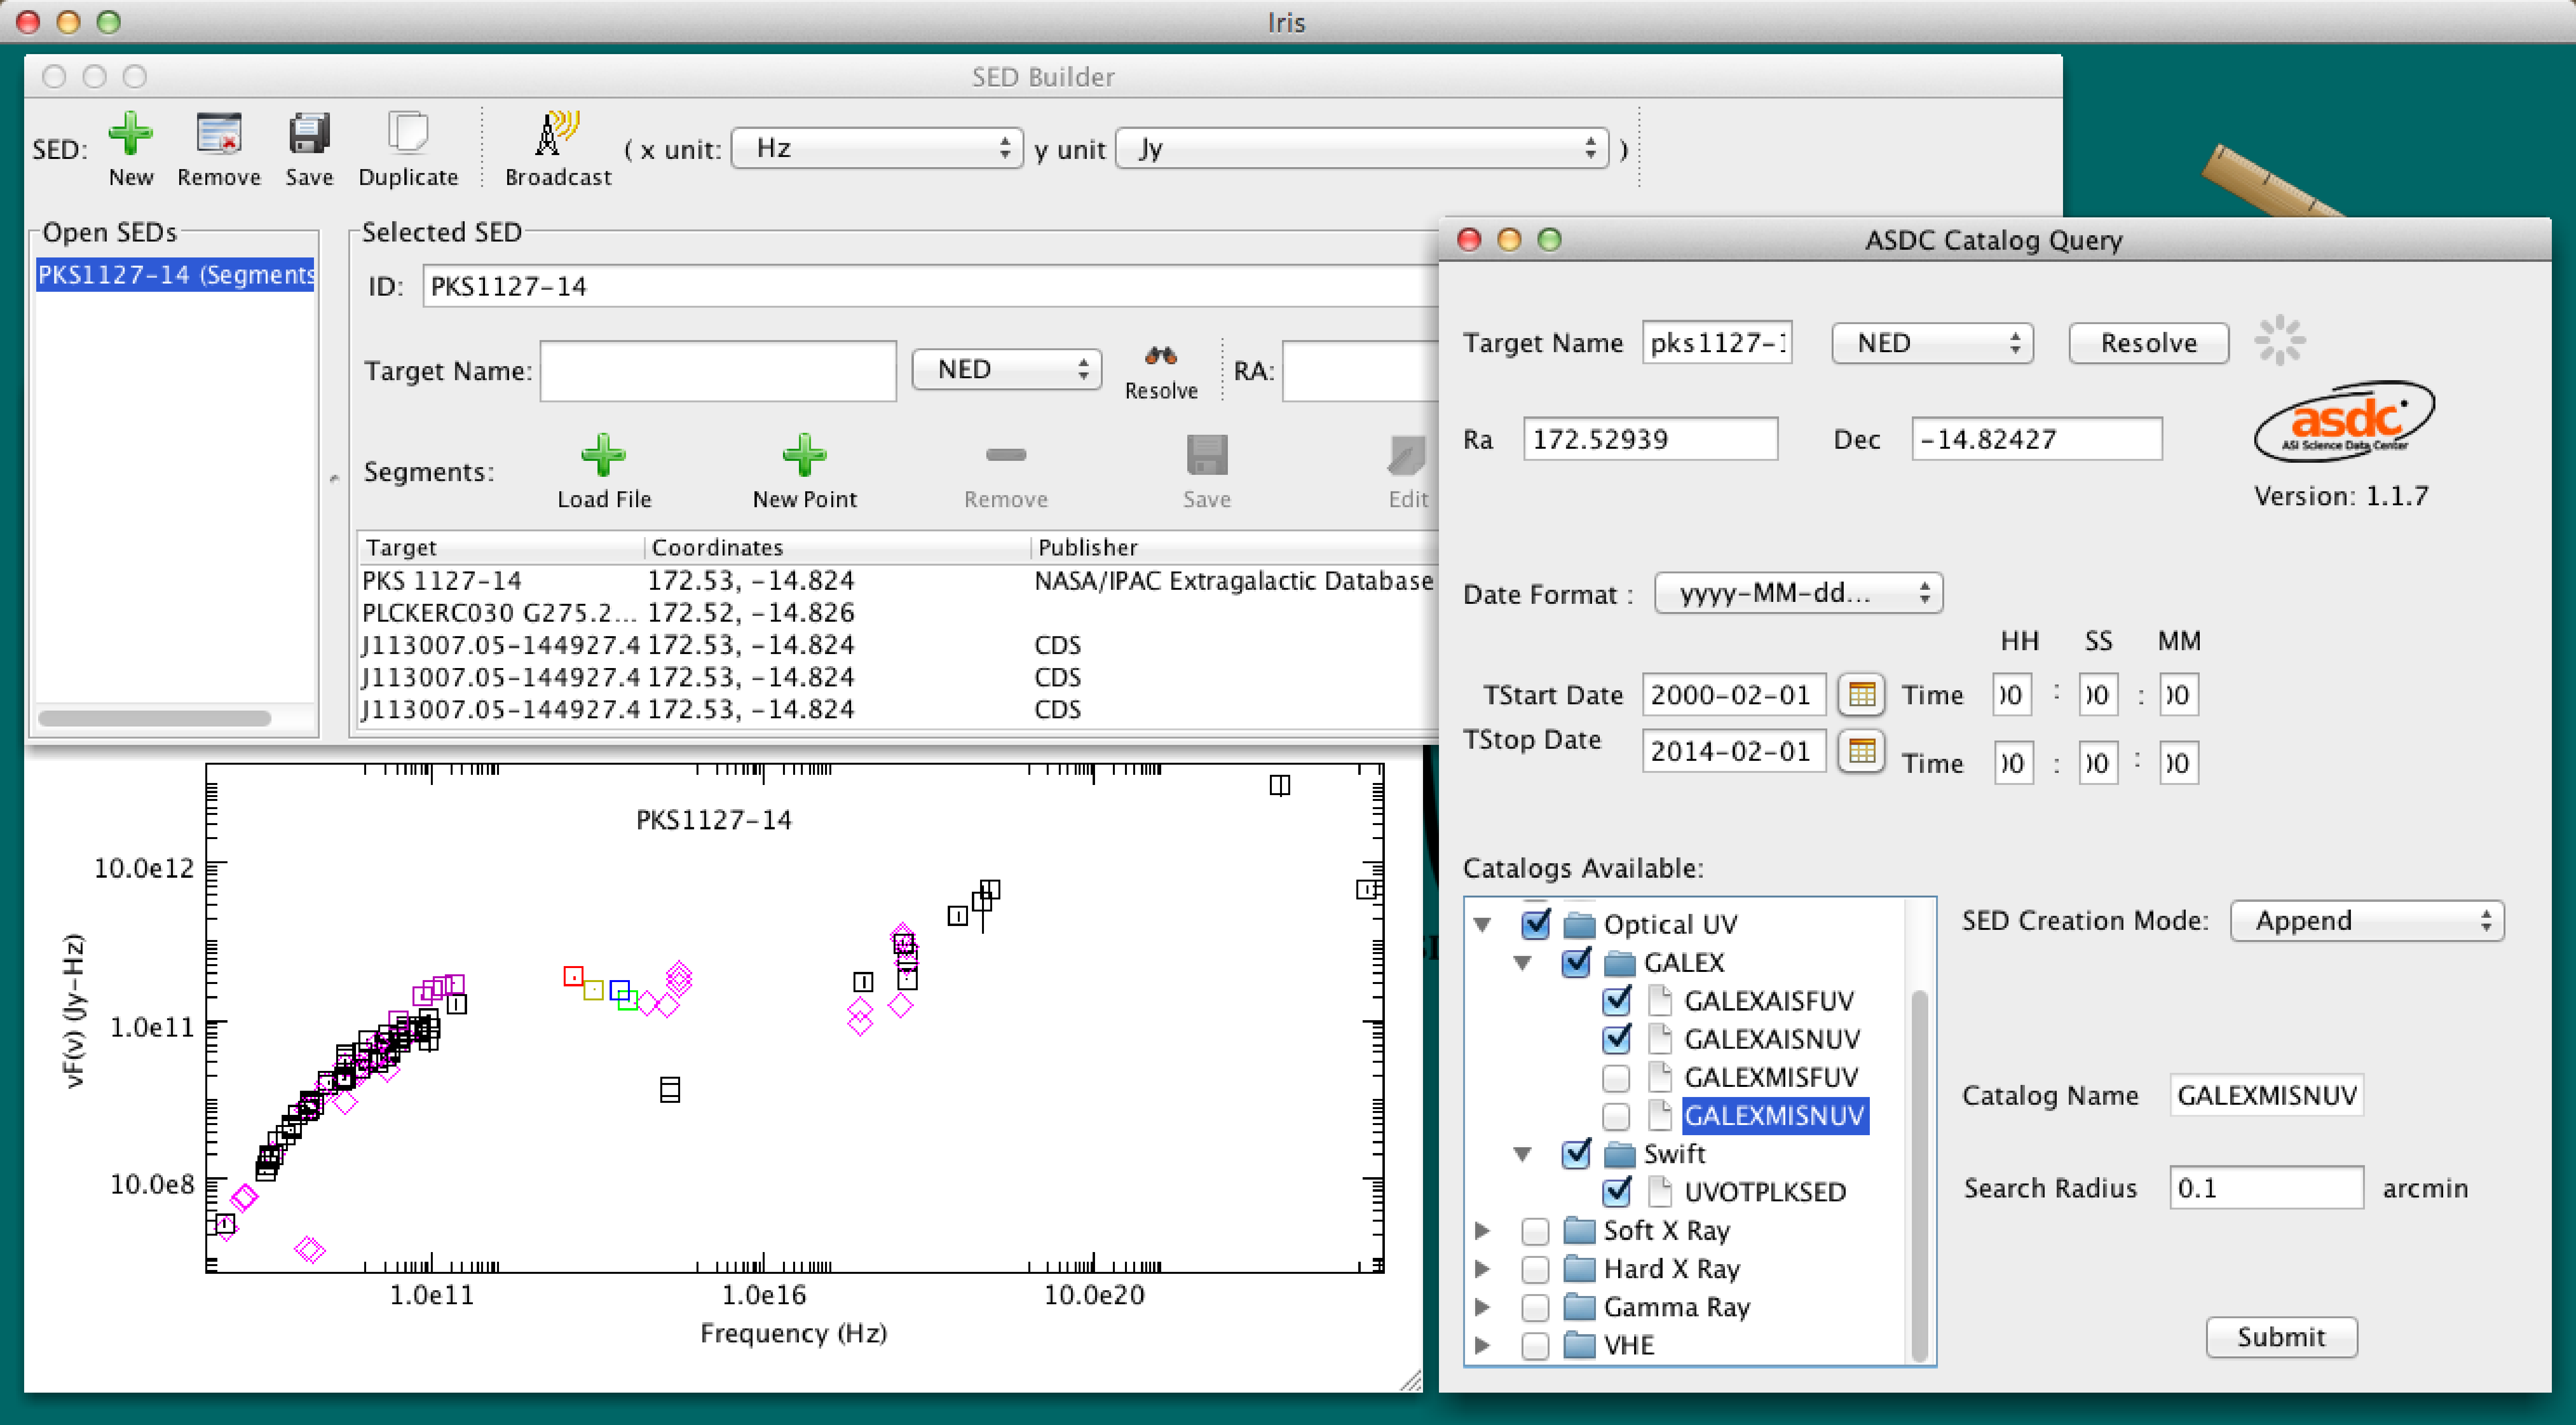
\includegraphics[width=0.7\columnwidth]{figures/built-in-visuals-loading1/built-in-visuals-loading1.png}
\caption{\textbf{\textit{\label{fig:load_data}} } Building the SED of blazar PKS 1127-14 in Iris. \textit{Top-left:} Data from the NED SED Service, a local file and from a SAMP message are managed in the SED Builder. \textit{Bottom-left:} The various data Segments plotted in $\mathrm{\nu F \left( \nu \right)}$ in the SED Viewier. Squares show data with flux uncertainties, whereas the pink diamonds denote points without associated uncertainties. Each Segment in the SED Bduilder is plotted in a different color. Black squares are the data taken from NED; the pink sqaures in the radio are the data from PLANCK; and the red, yellow, blue, and green sqaures in the near-IR are the for WISE bands. \textit{Right:} An ASDC Catalog Query form for PKS 1127-14. The user searches for data between specified dates and available instruments (Swift and GALEX in this case). The data may be added the open SED \texttt{PKS1127-14}.}
\end{center}
\end{figure}

\begin{figure}[h!]
\begin{center}
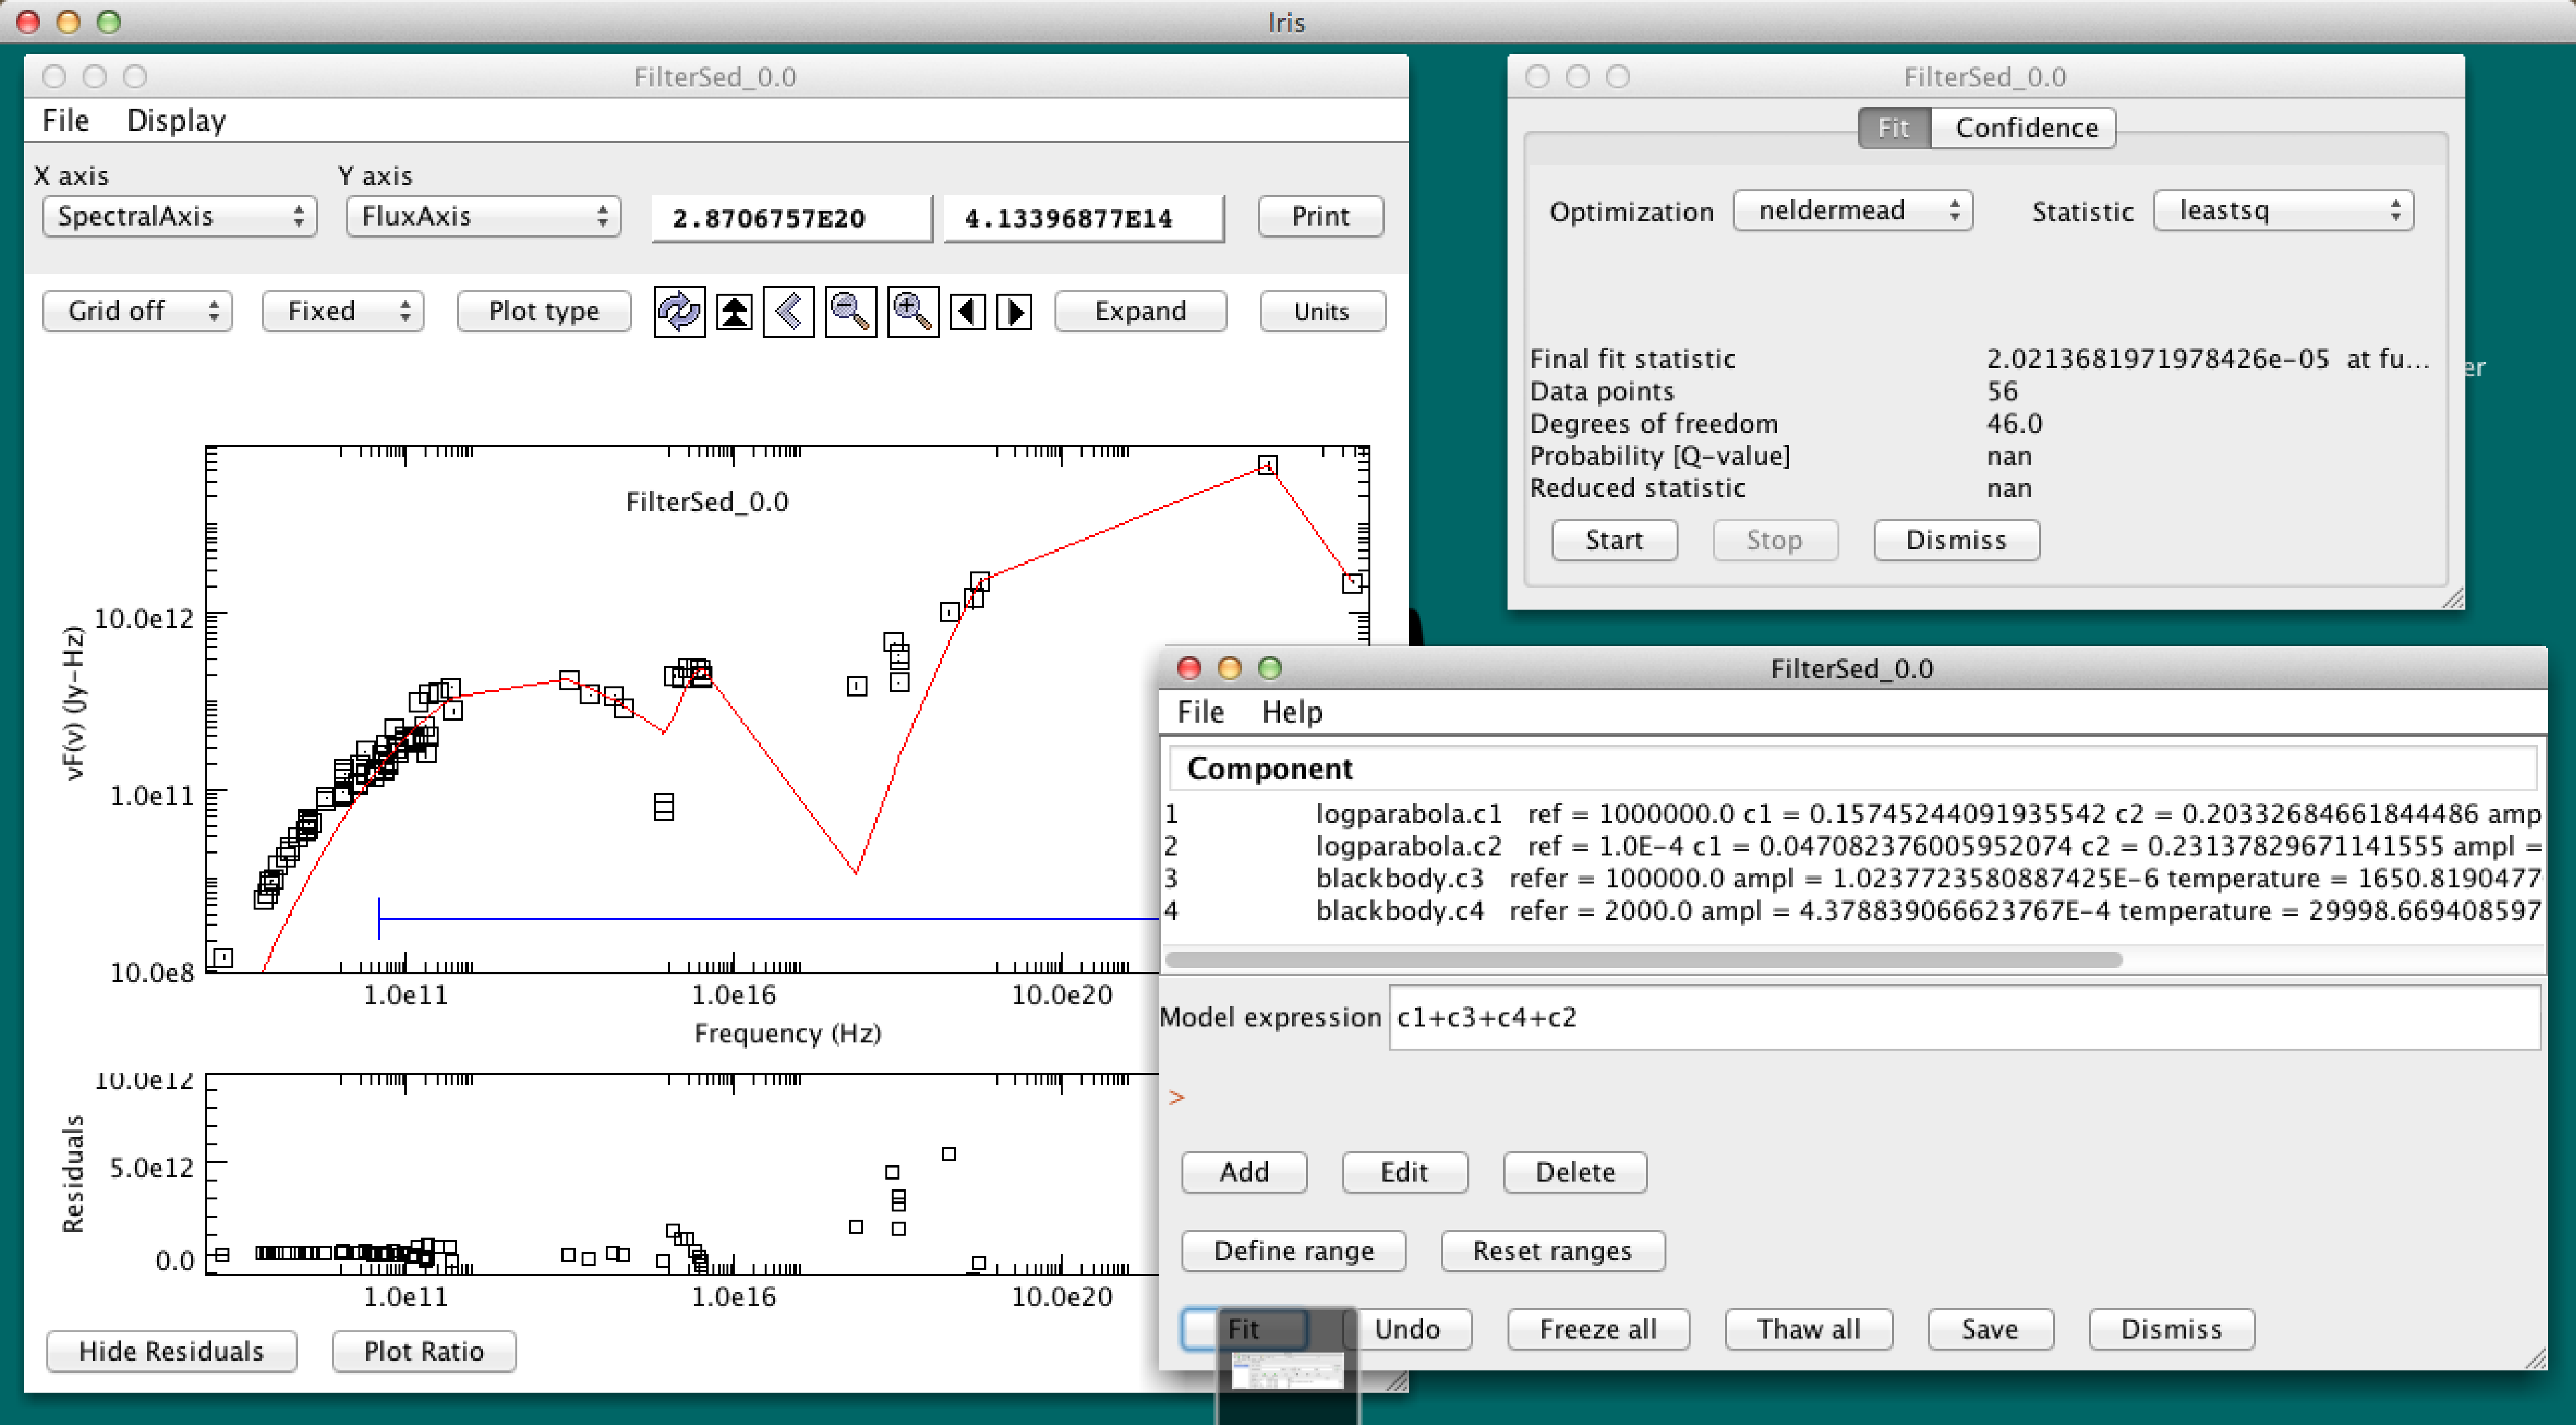
\includegraphics[width=0.7\columnwidth]{figures/fitting-1/fitting-1.png}
\caption{\textbf{\label{fig:fitting1} Fitting Visualization} Visualization of a linear combination of log-parabolas and blackbody distributions for FRSQ blazar PKS 1127-145, fit with Neldermead optimization and least-square statistics. \textit{Left:} The best fit linear combination overlaid on the SED data as a red curve. The blue line shows the spectral range over which the data was fit. Below the main plot are residuals of the fitted curve, in dex units. \textit{Top-right:} The fitting options and results. Here, the user chooses between Neldermead, Levenberg-Markwardt, and Monte-Carlo optimization and various least square and $\mathrm{\chi}^{2}$ statisitcs. The fit statistics are reported here after the fit has been performed. \textit{Bottom-right:} The Fitting Tool window. The model components used in the fit and their fitted parameter values are listed in the Components field. Below that is the Model Expression, in which the components are linearly combined. Note that components are referenced by the \textit{c\#} suffix of the component name.}
\end{center}
\end{figure}

\begin{figure}[h!]
\begin{center}
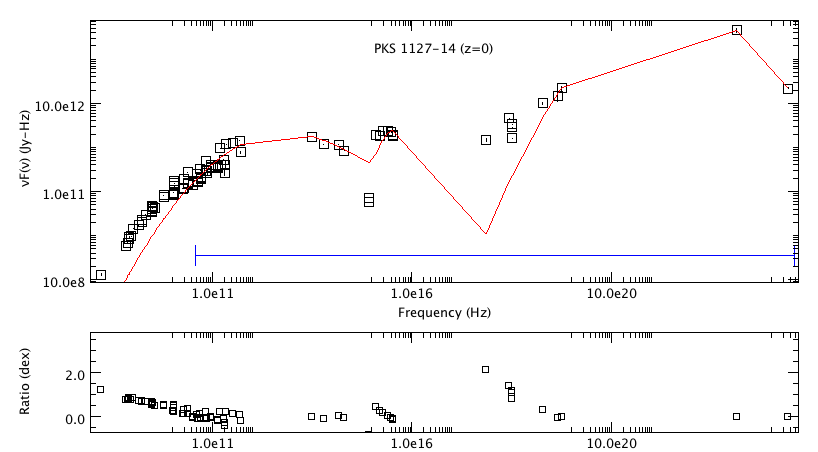
\includegraphics[width=0.7\columnwidth]{figures/all-models-plot-only2/all-models-plot-only2.png}
\caption{\textbf{\label{fig:fitting} Fitting Visualization} Visualization of a linear combination of log-parabolas and blackbody distributions for FRSQ blazar PKS 1127-145, fit with Neldermead optimization and least-square statistics. \textit{Top:} The best fit linear combination is overlaid on the SED data as a red curve. The blue line shows the spectral range over which the data was fit. \textit{Bottom:} The residuals of the fitted curve, in dex units.}
\end{center}
\end{figure}

\section{User Models and Templates}
\label{sec:usermodels}

Keeping with our requirements of developing an extensible SED analysis tool, we provide a user-end interface for adding custom models, templates, and template libraries for the fitting engine to use in a Custom Fit Models Manager.

Sherpa, Iris' fitting engine, provides \textbf{command line functions} for users to add their own models and templates to a Sherpa session. We wrap a GUI around Sherpa's \texttt{sherpa.astro.ui.utils} functions \texttt{load\_user\_model}, \texttt{load\_table\_model}, \texttt{load\_template\_model}, and \texttt{add\_user\_pars} for streamlined integration and user-friendliness. The user provides the full path to the directory where the models and templates exist, as well as information about the parameters. Installing a model saves a copy of the model files in the user's home directory (in \~{}/.vao/iris/components), allowing the user to apply the models in future sessions.

%; in this way, both users familiar or unacquainted with Sherpa will 

\subsection{Custom Python Functions}
Iris accepts custom models written as Python functions saved in *.py files. Any number of functions can be written in the file. The function must take two parameters: the first is an iterable of the model parameters, the second is a placeholder for the spectral axis, $x$, in units of Angstroms. For example, a model file for a modified black body
\(B_{\nu}(T) \left(\nu/\nu_{0}\right)^{\beta}\)
could be defined as in \textbf{Listing} \ref{lst:user_model_example}. User models can be arbitrarily combined with other custom or preset model functions.

\subsection{Table Models}
A table model is a single template, having just the $x$ and $y$ coordiantes. Iris accepts two-columned ASCII files as table models, following the convention where the first column is the spectral values (in Angstroms) and the second contains the fluxes (in $\mathrm{photons}/\mathrm{s}/\mathrm{cm}^{2}/{\AA}$). The fit returns the normalization constant (or amplitude) of the model.

\subsection{Template Libraries}
The template model is essentially a list of table models with parameters other than the amplitude. Like the \texttt{load\_template\_model} function in Sherpa, the user must create an index file which lists the parameter values of the templates and the full path to the template those parameter values describe (see Listing \ref{lst:templateconfig} for an example). Sherpa uses a grid-search method to find the best-fit template.

\begin{figure}[h!]
\begin{center}
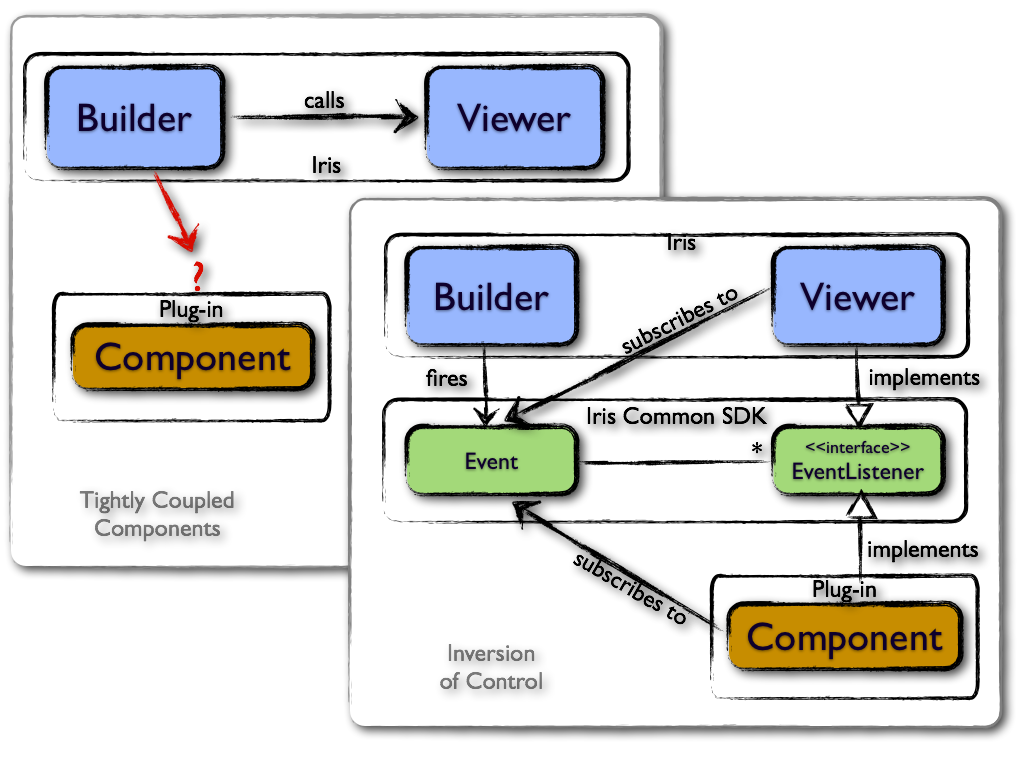
\includegraphics[width=0.7\columnwidth]{figures/IrisDiagrams.002/IrisDiagrams.002.png}
\caption{Inversion of Control}
\end{center}
\end{figure}

\section{A loosely coupled, event-driven, extensible architecture}
\label{sec:architecture}

As mentioned before, Iris was designed to put together existing and newly developed software components in a rich, extensible application. Also, Iris was developed by a distributed team.

In order to minimize the risk deriving from such constraints, we backed Iris with a loosely coupled architecture through a design pattern called Inversion of Control \citep*{ioc}.

But it was not just a matter of risk management: this design pattern also supports the implementation of ``liquid requirements'', i.e. a finite set of predetermined requirements plus an undefinite set of custom requirements to be implemented by users, at least in some simple cases, or, for more advanced features, by third party developers.

The architecture supporting the implementation of such requirements has different components that can be mapped to the Model-View-Controller (MVC) design pattern:
\begin{description}
\item[SEDLib] a basic I/O library provides classes the Model components of MVC. Unsurprisingly, SEDLib does so by implementing a Data Model specification defined by the IVOA. Such specification defines both the logical breakdown of spectral datasets, and the serialization in some standard file formats. So, on one end, SEDlib can perform the basic read/write operations on spectrophotometric files, while on the other it provides the data structures that client components can use and exchange.
\item[SEDManager] The MVC Controller role is played in Iris by the SEDManager, which is itself defined as an Interface. The manager works as a data storage for SEDLib instances that the different Iris components can share.
\item[Components] The actual Iris functionality is implemented by the Iris Components. They can be seen as the Views in the MVC pattern (or, more generally, they can provide any number of Views), since they present to the user the data stored in the Controller, query the Controller itself, and act upon the Models, i.e. the SED objects provided by SEDLib.
\item[Events] Views can be notified of changes in the Models by Events, if they implement the relative Listener interface and have been registered to the Events Queue. Events usually have a payload with more information about their content, and a pointer to the Model instances involved.
\end{description}

In summary, Components (Views) can be completely disentangled from each other and interact indirectly through the sole common interface represented by the SEDManager (Controller), which in turn stores the SED objects (Model). Dynamic changes in the system are notified to all interested agents (Listeners) via specific Events.

Components are thus agents that cohoperate by attaching themselves to a common \emph{bus} where the SEDManager provides the memory, and Events guarantee the flow of information.

\subsection{Inversion of Control}
We achieve loose coupling by an extensive use of Java Interfaces: components, events, and event listeners, for example, are all defined by interfaces whose implementation can, to some extent, be freely interchangeable.

Moreover, Inversion of Control is employed to decouple the implementation of components from the run time context: methods in the Interface are callbacks, and some of these callbacks get Interface-typed arguments which provide them context instances during the application execution. For this reason, this pattern is also sometimes referred to as \emph{Dependency Injection}.

Consider, for example, Iris Components: they are the main providers of Iris functionality, and they can correspond to buttons and menu items on the Iris desktop, loggers, data handlers, etc. They must implement the IrisComponent interface, which is listed in Listing \ref{lst:component}.

At startup the Iris application reads the list of Components to be initiated, and calls their \verb|init| call-back, which is in turn passed useful information like a reference to the SEDManager, or hooks to the application environment (more information is provided in the following sections).

The advantages of this architecture are both functional and non functional: it helped our heterogeneous developing team to work in a loosely coupled way, reducing the overall project risk, but it also provides the extensible framework we were seeking in the first place. As a matter of fact, plug-ins that can be loaded at run time (see section \ref{sec:plugins}) implement the same interfaces that the built-in components do (see section \ref{sec:components}), and they are instantiated exactly the same way. The only difference is in the timing: built-in Components get instantiated when the application itself is intialized, while plug-in can be instantiated (and discarded) at any time during the application execution.

\section{Iris Built-in Components}
\label{sec:components}

\subsection{SED Builder: SED I/O and Management}
\subsubsection{Data management: SEDs and Segments}
Users manage SEDs through the SED Builder (Figure~\ref{fig:sed_builder}). From the Builder, users can add, edit, remove, and save SEDs. Users can also beam data to other VO-enabled applications through SAMP messages from the Builder. Any number of SEDs can be analyzed in an Iris session. Each SED must have a unique identifier; by default, the first SED is named "Sed;" the second SED would be "Sed.1," the third "Sed.2," and so on. The user switches between SEDs by clicking on a SED name in the Open SEDs field; the visualizer will automatically update to the selected SED. 

SEDs are built and managed in Segments, which are groups of (spectral, flux) coordinates. For example, a spectrum is considered a Segment. The results of a NED SED Service query are also handled as Segment. Photometric points loaded from file, SAMP or from ASDC are managed as individual Segments (i.e. each photometric point is its own Segment). Clicking on a SED in the Open SEDs field will show all the Segments that populate that particular SED. SED Builder shows where the Segment data came from, the recorded RA and Dec of the Segment, and the number of points in the Segment. Segments can be handled separately from other Segments in the SED; users can add, edit, remove, and save selected Segments separately from the SED in which it lives. 

\subsubsection{Importing data}
The SED Builder handles SED I/O. As described in Section~\ref{sec:overview}, Iris accepts data from a variety of sources, and is lenient on the data format. Figure~\ref{fig:data_sources} illustrates that Iris imports data from built-in data archive portals as well as from outside resources like local files, URLs, other VO-enabled applications, and from plugins.

Iris natively supports IVOA-compliant FITS and VOTable formats (described in \cite{2012arXiv1204.3055M}). Files in these formats will automatically be added to SED Builder and the visualizer. The Builder can convert ASCII Tables, CSV, Tab-Seprated-Tables, IPAC tables\footnote{http://irsa.ipac.caltech.edu/applications/DDGEN/Doc/ipac\_tbl.html}, SAMP messages, and non-IVOA-compliant VOTable and FITS files into the native format with user input. We provide two file converted forms: (1) the Import Setup Frame, which handles spectrum-style files (i.e. those with columns for the spectral, flux and flux uncertainties), and (2) the Photometry Catalog Importer, which handles photometry catalogs (i.e. files where each column represents a passband and the values represent the fluxes). Users can save their setup options from the Import Setup Frame to a configuration file and automatically read-in files of the same format to Iris via the command line.

The SED Builder also has a hook for adding custom file filters. A user can develop a custom file reader that would convert a non-standard file, e.g. a SExtractor-type file, to an IVOA-compliant format. This kind of plugin would allow the user to automatically read-in non-standard files to Iris, without needing to use the importer tools (See Section~\ref{sec:plugins} for details on developing Iris plugins).

\subsubsection{Saving data}
Users can save entire SEDs or sets of Segments to IVOA-compliant VOTable or FITS files. By default, Iris will save the data and all of its associated metadata in VOTable format. This means if the SED is composed of more than one Segment, the individual Segments will remain when we re-read the data back into Iris. These files may be difficult to read into other tools. Therefore, we provide a simpler output format that saves the most important information: the spectral, flux and flux uncertainties, along with data point reference IDs and a column of the original flux (useful if an aperture correction was applied to any point). All Segment distinctions dissappear, along with the metadata, making the data more compliable for use in external applications. The user supplies the desired X and Y units for the new SED from the drop-down menus, converting all data to the same units.

\subsection{Science Tools}
We provide built-in science tools that perform calculations commonly used in SED analysis: redshifting, interpolation, and integration. The data is setup on the Java-side of Iris, but the actual calculations are done in Sherpa. For this, we implement the \textbf{sherpa-samp interface}, which links the Java implementation of SED Builder to the Python implementation of the SED science tools in Sherpa through SAMP interfaces (for more details on sherpa-samp, see Section~\ref{subsec:sherpa}).

The open SEDs are listed in the Science Tools frame. The user selects the SED they wish to analyze, and inputs the required information for a calculation.

\subsubsection{Redshifting}
Redshifting an SED in Iris refers to cosmological redshift. Because the apparent magnitude of a source is dimmer at high redshifts than low redshift, we correct the flux so that the area under the shifted SED equals that of the un-shifted SED:

\begin{equation} \label{eq:redshift}
f_{z_{final}}(\lambda) = f_{z_{initial}}(\lambda) \frac{\sum_{k=1}^N (f_{z_{initial}}(\lambda_{k+1})+f_{z_{initial}}(\lambda_{k}))}{\sum_{k=1}^N (f_{z_{final}}(\lambda_{k+1})+f_{z_{final}}(\lambda_{k}))}
\end{equation}

In sherpa-samp, we extend the astLib\footnote{http://astlib.sourceforge.net/} \textit{astSED} class which implements Equation~\ref{eq:redshift}. 

From the user's perspective, he/she supplies the initial and final redshift of the SED and clicks "Create New SED." The returned SED has the same name of the unshifted SED, appended with ``\_redshift.'' For example, if the final redshift is \(z=0.0\) the shifted SED is named "Sed\_0.0."

\subsubsection{Interpolation}
Iris provides 1D interpolation along the spectral axis. There are three interpolation options: linear, linear spline, and nearest neighbor. Interpolation may be carried out on a linear or logarithmic scale. Users may choose the number of bins, the spectral range overwhich to interpolate, and may choose to smooth the resultant SED via a boxcar method.

\subsubsection{Integration}
The Integration tool was developed to make estimating integrated fluxes of a SED quick and painless. Iris provides two methods of integration: (1) through a user-defined passband, and (2) through a photometric filter. The first option lets the user specify the spectral range in wavelength, frequency, or energy units (Angstroms, Hz, and keV, respectively) to integrate under. The second estimates the integrated flux measured through any of the photometric filters provided by the Spanish Virtual Observatory's (SVO's) Filter Profile Service\footnote{http://svo2.cab.inta-csic.es/theory/fps/index.php} \cite{2013arXiv1312.3249S}. We chose the SVO's Filter Profile Service because of its extensive collection (over 1000 filters at IR, optical and UV instruments) and of its VO-compliancy. The user chooses from a list of filters which can be searched by double-clicking on an instrument name, or by searching for a string in the browser. The user sees the min, max and effective wavelengths of the filters before applying the filter to the SED.
How does it work in the background??
Both methods return the effective wavelength of the passband in Angstroms and the calculated flux in Janskys. The user can export the data to a new SED or save the results to a FITS or VOTable file.

\subsection{Sherpa}
\label{subsec:sherpa}





\begin{figure}[h!]
\begin{center}
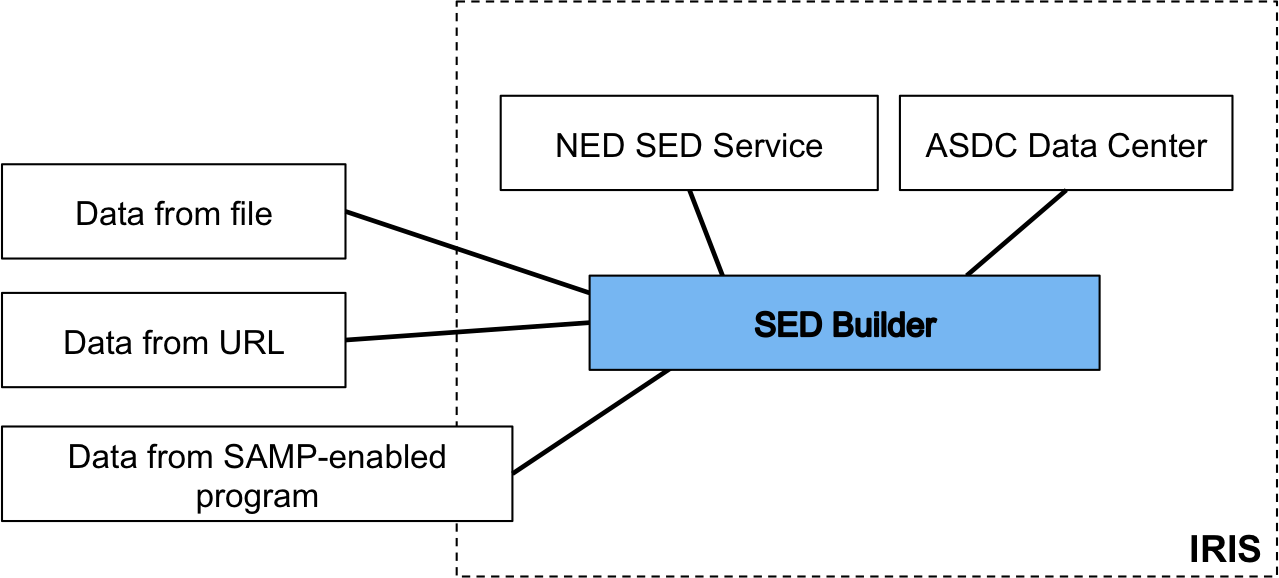
\includegraphics[width=0.7\columnwidth]{figures/iris_data_sources2/iris_data_sources2.png}
\caption{\textit{\textbf{\label{fig:data_sources} Available Data Sources}}\textit{}\textbf{}\textit{} Users may import data from the built-in data archive services: NED SED Service and the Italian Space Agency Science Data Center (ASDC). Data may also be uploaded from a local file, a URL, a SAMP message from a VO-enabled program (like TOPCAT, CDS Photometry Viewer, or the Data Discovery Tool), or through a custom file filter plugin at run time.}
\end{center}
\end{figure}

\begin{figure}[h!]
\begin{center}
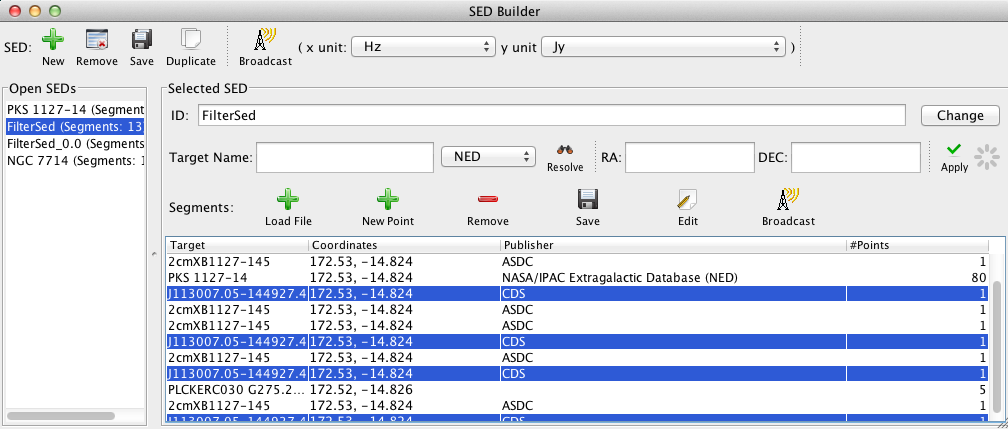
\includegraphics[width=0.7\columnwidth]{figures/sed_builder/sed_builder.png}
\caption{\textit{\textbf{\label{fig:sed_builder} SED Builder}} An example view of the SED Builder. On the right side of the window is a list of SEDs open for analysis; in this case, \textit{FilterSed} is selected. The Segments or components that constitute \textit{FilterSed} are shown in the Segments section. Segments may be managed separately. Highlighed SEDs or Segments may be edited, removed, saved or broadcast to an external SAMP-enabled application. New Segments and SEDs are added to the Iris session through the SED Builder. }
\end{center}
\end{figure}

\begin{figure}[h!]
\begin{center}
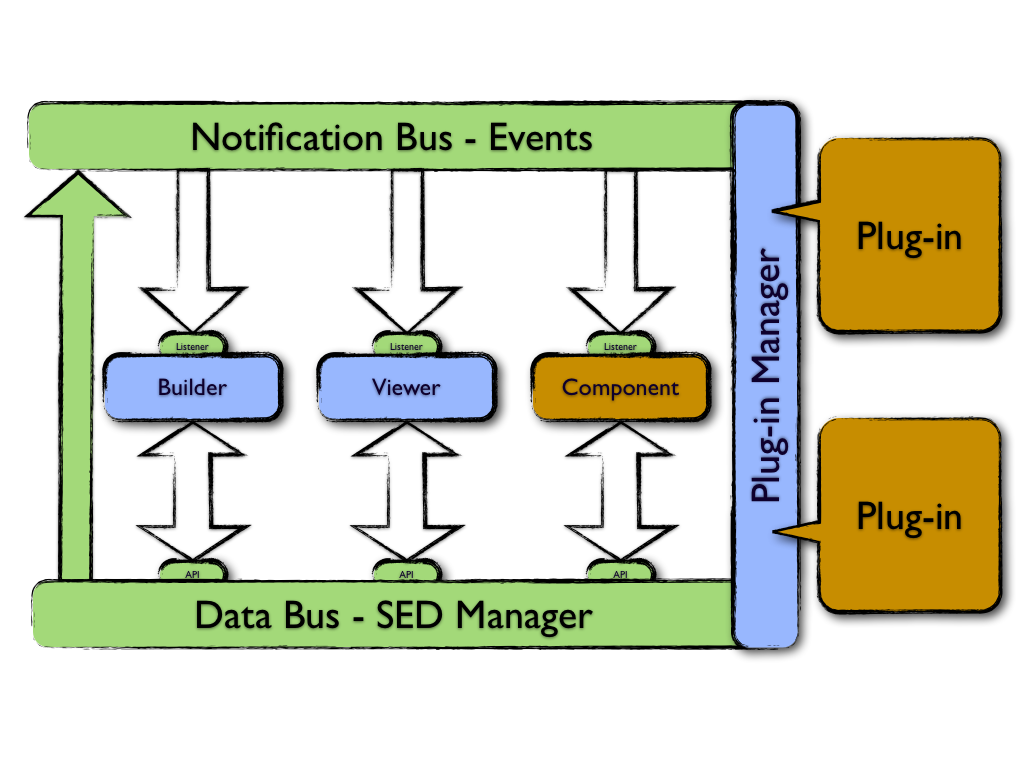
\includegraphics[width=0.7\columnwidth]{figures/IrisDiagrams.1/IrisDiagrams.1.png}
\caption{Replace this text with your caption}
\end{center}
\end{figure}

\section{Plug-ins: the Software Development Kit}
\label{sec:plugins}

Iris offers a Software Development Kit (SDK) that can be used to extend the Iris capabilities through the use of dynamically pluggable add-ons, or plug-ins.
The use cases for this are basically two:
\begin{description}
\item[New functionality] A developer may want to create SED-related capabilities in one or more new Components. This use case can be broken down in more detailed and concrete extensions, described later in this section.
\item[Custom-to-Standard adapters] A developer may want to create adapters that query a non-standard service, or load a non-standard data set, and then turn the data to SEDLib objects, thus effectively standardizing them so that they can be used by other components in the Iris environment, or reused by other VO-compliant applications. In other terms, one can achieve interoperability using the Iris infrastructure starting from a non-interoperable service, file, or tool. Iris actually has some built-in Custom-to-Standard adapters, like the sherpa-samp layer described in section \ref{sec:components}, or the ASDC plug-in interface that queries a quasi-standard service, described in section \ref{sec:asdc}.
\end{description}

\subsection{Anatomy of a Plug-in}
A single Jar file can archive several plug-ins, and each plug-in can bundle several Iris Components.

Each Component can provide several additions to Iris, as described in some detail below:

\subsubsection{Menus and Buttons}
Usually, although not always, an Iris Component is visible to the user as either a set of buttons on the Iris Desktop, or as a set of menu items in the Iris menu bar, or both.

Menu items can be added to either the File menu or to the Tools menu in a specific plugin-related folder.

While the implementation of such buttons and menu items could be done from scratch by implementing some Java Interfaces, a set of abstract classes implements a lot of the boiler plate code and makes some convenient assumptions. This way buttons and menu items can be created with very few lines of code.

Menu items and buttons can be customized by providing the button name, a description that will be rendered as a mouse-hover tooltip, and icons.

\subsubsection{Command Line}
Iris offers a framework for providing simple command line interfaces to its tools. For example, Iris ships a command line interface to the SED Builder (see Section \ref{sec:components}) that allows users to import non-standard files in bulk through scripts, possibly starting from templates saved interactively from the SED Builder.

This framework is extensible through a simple dispatching mechanism. Each component has a name that is used to dispatch the command line argument to the right CLI engine. For instance, the line \verb|./Iris builder config.txt| instructs Iris to dispatch the \verb|config.txt| argument to the SED Builder's CLI engine.

Components bundled with plug-ins can provide such an engine by implementing the ICommandLineInterface Java Interface (see Listing \ref{lst:cli}).

\subsubsection{SAMP Handlers}
A possible extension that plug-ins can offer to the users is SAMP Handlers: when Iris receives a SAMP message that matches the Handler's \verb|mtype|, the message is directly dispatched to the Handler itself by the Iris framework. As a matter of fact, Iris just offers a convenient shortcut to the excellent STIL implementation of SAMP, leveraging one of the best SAMP library available, and making it available to the users with just the bare minimum amount of work required: the setup of the SAMP infrastructure through STIL is all done by Iris, including a keep-alive mechanism that brings a SAMP Hub up if one is shutdown.

A hook is provided for Components willing to send their own SAMP messages to the SAMP Hub, again as a convenient shortcut to STIL.

\subsubsection{Custom Events}
The Iris Events Framework is itself extensible: this way Plug-ins can, if needed, create their own nested loosely coupled architecture for their own Components.

\subsubsection{SED attachments}
Components can attach arbitrary objects to the SEDs managed by the SEDManager. This way they do not have to independently manage the additional information they might want to store about the individual SEDs. When SEDs are deleted, the manager takes care of releasing any references to the attachments, so to avoid memory leaks.



\subsection{Plug-in examples}
\subsubsection{ASDC - stable}
The Italian Space Agency Science Data Center (ASDC) hosts a database with tens of catalogs in a very wide range of wavelengths, also providing time domain information.

A plug-in for providing Iris with a rich graphical user interface to query their database was developed by the ASDC in a collaboration between the ASDC and the Iris teams. The plug-in became part of the main Iris distribution in v2.0 and provided a valuable test bench to review, validate, and improve the Iris Software Development Kit.

While the ASDC data query tool is now part of the Iris distribution, it still provides a very good example of how a plug-in can be integrated seamlessly in the Iris framework to add specific value to it. Integration can be so seamless, actually, that including the plug-in into the main Iris distribution is almost exclusively a matter of configuration than of coding.

The ASDC data query tool extends the capabilities of the SED Builder by providing a rich graphical user interface that allows users to check what archives to query, and since the ASDC query is a positional cone search, the client provides different adjustable search radii for each catalog which default to reasonable values consistent with the resolutive power of the individual instruments.

Moreover, the tool allows to query for specific observation time ranges, thus allowing basic time domain analysis of the SEDs.

This component proves several points about the Iris framework and SDK:
\begin{description}
\item[Custom-to-Standard adapters] The ASDC web service backing up the implementation of the query tool does not comply with any VO data access protocols (at least not yet), as it was designed as a private interface to their database to be consumed by a dedicated client. The client on the Iris desktop assumes that the service implements the private interface, and can query it. The data files coming from the service, on the other hand, are actually compliant with the IVOA specifications, so they can be directly read by SEDLib and passed to the SEDManager.
\item[Agents loosely coupled interoperability] Although the ASDC plugin was not designed as part of Iris, it integrates seamlessly with the Iris built-in components. When the ASDC query tool instantiates an SED from the service, this gets listed in the SED Builder and visualized in the SED Viewer, even though it does not interact directly with any of them: they all interact only with the SED Manager and they get notified of changes by the events that are fired when Models are changed.
\item[The Iris SDK] As it will be explored in some detail in section \ref{sec:writeplugin}, a plug-in developer can pretty much focus on the implementation of her components' business logic, without worrying too much about the boiler plate code required to configure such components. By using the abstract classes that the Iris framework
provides, one can leverage the existing components with just a few lines of code and then start adding value to the entire application.
\end{description}

\subsubsection{Vizier - experimental}
\label{sec:asdc}
Experimental plug-ins are shipped with Iris but they can only be activated by turning on switches on the Iris command line. For instance, if one starts Iris with the command \verb|./Iris --vizier| an experimental plugin for the CDS Vizier photometric service gets loaded in the usual Iris desktop.

While this component is, at the time of this writing, still experimental, it shows some properties of the Iris framework and SDK.

As for the ASDC plug-in, this component shows that one can use Iris and its framework to rapidly build an adapter from a dedicated service interface, leveraging the particular specs of the service, so to make datasets interoperable with the other Iris tools, third party plug-ins, and possibly other VO tools.

\subsubsection{R - experimental}
A highly experimental proof-of-concept plug-in was developed to explore the possibility of interfacing Iris with rich analysis environments like R. The plug-in shows how one can \emph{beam} data from Iris to R and trigger some analysis on the dataset in R.


\subsection{Other Extensibility Points}

\subsubsection{Custom File Readers}
Iris supports a fair number of {fi}le formats natively: VOTable,
FITS, CSV, TSV, ASCII, and IPAC tables. However, new {fi}le {fi}lters can be created and
loaded at runtime. One can also create {fi}lters for the natively supported {fi}les: in this
case, the custom {fi}lter would parse the {fi}le and map the metadata to the IVOA Data
Model {fi}elds.

\subsubsection{Persistence}
Components can also get a handle to the configuration directory, usually a hidden folder in the user's home directory, if they need to persist information like user's preferences, local databases, or work sessions.



\subsection{How to write an Iris plugin}
\label{sec:writeplugin}
Iris uses Maven Archetypes to streamline the process of building and distributing Iris plug-ins.

You might also write plug-ins without using Maven, but you would need to take care of many steps that the Maven-generated project automatically takes care of, like the inclusion of your dependencies in your plug-in's jar file.

In order to have a test plugin up and running you just need to create a new project from the Maven archetype and package it:
\begin{verbatim}
$ mvn archetype:generate\
        -DarchetypeRepository=http://vaotest2.tuc.noao.edu:8080/artifactory/ \
        -DarchetypeArtifactId=iris-plugin-archetype \
        -DarchetypeGroupId=cfa.vo \
        -DarchetypeVersion=1.1
\end{verbatim}

The above command will ask you some questions about the metadata for your plug-in project, like the group id, the project id (called artifact-id in Maven), and the version. At the end of the process you should have a directory named after your project-id. This directory contains all the files needed to build and package a test plugin.

You can type \verb|mvn package| from the newly created directory and Maven will package the test plug-in for you in the \verb|target| directory as a jar file.

You can use the Iris Plugin Manager component to install this jar file into Iris. As soon as you do it, a new button should appear on the Iris desktop. If you click on it, a rather impressive dialog box with the universal salutation ``Hello World!'' should appear on your screen.

You can inspect the source code of this project and notice that most of it is made of metadata strings and basic class definitions and instantiations. By inheriting from the abstract classes that are provided with the Iris SDK, the actual code that one needs to implement starts from the implementation of the \verb|onClick| callback of the AbstractPluginMenuItem class. From that call on, a plug-in developer can focus on the implementation of their components and start using the hooks provided by the Iris Framework in order to interoperate with the other Iris components, and possibly with other VO applications.

One can start from this dummy project, inspect the source code, make changes to the package and class names and to the metadata strings, and then start implementing their component's business logic and user interface.

The Iris website has a somewhat extensive documentation on how to write plug-ins, and you can contact the authors of this paper for further information.

\section{Conclusion}
\label{sec:conclusion}

To summarize, Iris provides:
\begin{itemize}
\item built-in capabilities for building, viewing, and analyzing broad-band spectro-photometric SEDs;
\item seamless integration between existing and new code in Python and Java;
\item a python framework for fitting user provided models and templates;
\item interoperability with virtual observatory tools through the Simple Messaging Application Protocol (SAMP);
\item a Java Software Development Kit (SDK) that allows developers to extend the Iris functionalities.
\end{itemize}

\section{Code Snippets}
\subsection{IrisComponent interface}
\label{lst:component}
\begin{verbatim}
/**
 * Copyright (C) 2012 Smithsonian Astrophysical Observatory
 *
 * Licensed under the Apache License, Version 2.0 (the "License");
 * you may not use this file except in compliance with the License.
 * You may obtain a copy of the License at
 *
 *         http://www.apache.org/licenses/LICENSE-2.0
 *
 * Unless required by applicable law or agreed to in writing, software
 * distributed under the License is distributed on an "AS IS" BASIS,
 * WITHOUT WARRANTIES OR CONDITIONS OF ANY KIND, either express or implied.
 * See the License for the specific language governing permissions and
 * limitations under the License.
 */

/*
 * To change this template, choose Tools | Templates
 * and open the template in the editor.
 */

package cfa.vo.iris;

import java.util.List;
import org.astrogrid.samp.client.MessageHandler;

/**
 *
 * Interface implemented by Iris components. By implementing this interface the components
 * allow the framework to retrieve the information needed to run and initialize them.
 *
 * @author olaurino
 */
public interface IrisComponent {
    /**
     * This method is invoked to initialize the component. If the component has to launch windows, frames or
     * background services, this is the right method to do so. Otherwise the component will be called only if a callback
     * is invoked.
     *
     * @param app A reference to the running application
     * @param workspace A reference to the application's workspace
     */
    void init(IrisApplication app, IWorkspace workspace);
    /**
     * Return the name of this component. This name might be listed in a widget along with the other registered components.
     * @return The component's name as a String.
     */
    String getName();
    /**
     * Get e description for this component. The description might be listed in a widget along with the other
     * registered components.
     *
     * @return The component's description as a String.
     */
    String getDescription();
    /**
     * Get a command line interface object for this component.
     * @return A CLI object
     */
    ICommandLineInterface getCli();
    /**
     * Initialize the Command Line Application interface
     * @param app Reference to the enclosing application
     */
    void initCli(IrisApplication app);
    /**
     * The component can contribute menu items and desktop buttons to the enclosing GUI applications
     * by providing a list of MenuItems.
     *
     * @return A list of the menu items this component will contribute to the application.
     */
    List<IMenuItem> getMenus();
    /**
     * The component can register any number of SAMP message listeners by providing a list of them.
     *
     * @return A list of the SAMP message listeners that have to be registered to the SAMP hub.
     */
    List<MessageHandler> getSampHandlers();

    /**
     * Callback invoked when the component is shutdown
     */
    void shutdown();
}
\end{verbatim}

\subsection{Command Line Interface} \label{lst:cli}
\begin{verbatim}
/**
 * Copyright (C) 2012 Smithsonian Astrophysical Observatory
 *
 * Licensed under the Apache License, Version 2.0 (the "License");
 * you may not use this file except in compliance with the License.
 * You may obtain a copy of the License at
 *
 *         http://www.apache.org/licenses/LICENSE-2.0
 *
 * Unless required by applicable law or agreed to in writing, software
 * distributed under the License is distributed on an "AS IS" BASIS,
 * WITHOUT WARRANTIES OR CONDITIONS OF ANY KIND, either express or implied.
 * See the License for the specific language governing permissions and
 * limitations under the License.
 */

/*
 * To change this template, choose Tools | Templates
 * and open the template in the editor.
 */

package cfa.vo.iris;

/**
 * A simple interface for providing CLI access in an extensible, pluggable way
 * @author olaurino
 */
public interface ICommandLineInterface {
    /**
     * The name that has to be associated with the implementing component.
     * When the calling application parses the command line, it will interpret the
     * first argument as the component to which the command has to be relayed, using this string
     * as a key.
     *
     * @return The compact name that identifies this CLI
     */
    String getName();
    /**
     * Callback that gets called when a command line is parsed and associated to the implementing component.
     *
     * @param args The command line arguments.
     */
    void call(String[] args);
}
\end{verbatim}

\subsection{User Model Example} \label{lst:user_model_example}
\begin{verbatim}
import numpy as np

def modified_blackbody(p, x):
    """
    Modified blackbody of the form:
    A * B_lambda(T) * (c / (lambda / lambda_0))**beta

    Parameters
    ----------
    p : [lambda_0, A, temp, beta]

        p[0] 'lambda_0' : refernce wavelength
        p[1] 'A' : amplitude of model at reference wavelength
        p[2] 'temp' : temperature of blackbody
        p[3] 'beta' : dust emissivity index

    x : array
        spectral values, in Angstroms
    """
    
    # blackbody function, in terms of wavelength (in Angstroms)
    c1 = 1.438786e8  # in AA K
    efactor = c1 / p[2]
    numerator = p[1] * np.power(p[0], 5.0) * (np.exp(efactor / p[0]) - 1.0)
    denominator = np.power(x, 5.0) * (np.exp(efactor / x) - 1.0)
    B_lambda = numerator / denominator

    # speed of light in Angstroms/second
    c = 2.998e18

    powerlaw = (c / (x/p[0]))**p[3]

    return B_lambda * powerlaw
\end{verbatim}

\subsection{Template Configuration File} \label{lst:templateconfig}
\begin{verbatim}
# INDEX REFER MODELFLAG FILENAME
0.0     5000  1   /home/user/iris-2.0.1-unix-x86_64/examples/sed_temp_index-0.00.dat
-0.10   5000  1   /home/user/iris-2.0.1-unix-x86_64/examples/sed_temp_index-0.10.dat
-0.25   5000  1   /home/user/iris-2.0.1-unix-x86_64/examples/sed_temp_index-0.25.dat
-0.35   5000  1   /home/user/iris-2.0.1-unix-x86_64/examples/sed_temp_index-0.35.dat
-0.50   5000  1   /home/user/iris-2.0.1-unix-x86_64/examples/sed_temp_index-0.50.dat
\end{verbatim}

\bibliography{aciris.bib}

\end{document}

